% THIS IS DEPRECATED! USE SUBFIG INSTEAD!


\documentclass[10pt]{article}
\usepackage{subfigure}
\usepackage{graphicx}
\usepackage{float} % to use [H] placement

\begin{document}
\section{Test Graphics}

In Figure \ref{fig:SingleFigure1} we show something.
%single figure
\begin{figure}[ht!]
\begin{center}
\fbox{\rule{0pt}{2in} \rule{0.9\linewidth}{0pt}}
\end{center}
   \caption{Example of caption.}
\label{fig:SingleFigure1}
\end{figure}

In Figure \ref{fig:subfigureExample} we show three things. In \subref{fig:subfig1} we show the first thing, in \subref{fig:subfig2} we show the second thing, and in \subref{fig:subfig3} we show the third thing. In \ref{fig:subfig1} we do something.
%multiple figures
\begin{figure}[ht!]
\centering
\subfigure[Caption of subfigure 1]{
\fbox{\rule{0pt}{2in} \rule{0.2\linewidth}{0pt}}%box
%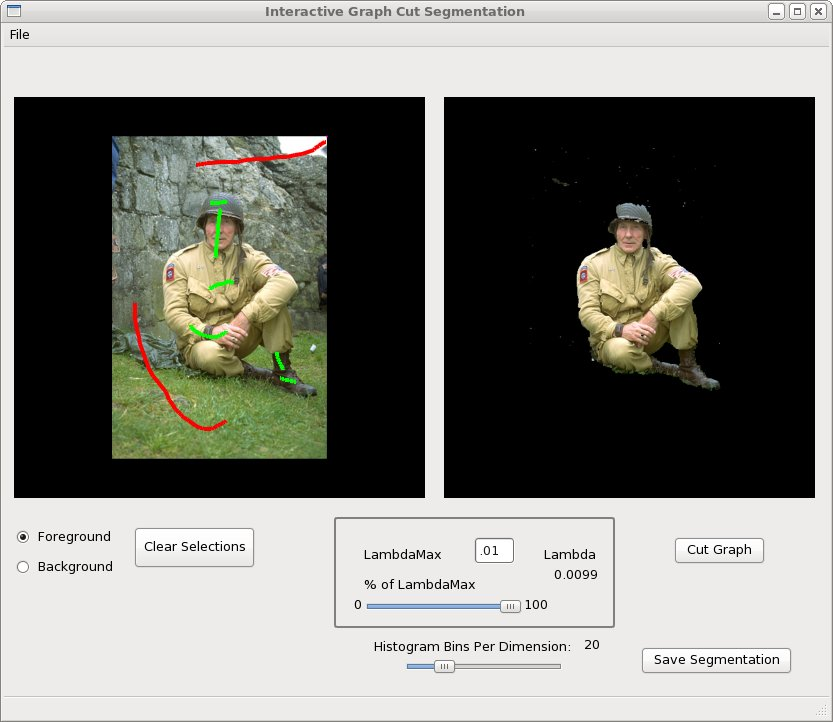
\includegraphics[width=0.4\linewidth]{Soldier}%actual image
\label{fig:subfig1}
}
\subfigure[Caption of subfigure 2]{
\fbox{\rule{0pt}{2in} \rule{0.2\linewidth}{0pt}}
\label{fig:subfig2}
}
\subfigure[Caption of subfigure 3]{
\fbox{\rule{0pt}{2in} \rule{0.2\linewidth}{0pt}}
\label{fig:subfig3}
}
\caption[Optional caption for list of figures]{Caption of subfigures \subref{fig:subfig1}, \subref{fig:subfig2} and \subref{fig:subfig3}}
\label{fig:subfigureExample}
\end{figure}

In Figure \ref{fig:SingleFigure2} we show something else.
%single figure
\begin{figure}[ht!]
\begin{center}
\fbox{\rule{0pt}{2in} \rule{0.9\linewidth}{0pt}}
\end{center}
   \caption{Example of caption.}
\label{fig:SingleFigure2}
\end{figure}


\end{document}
